\documentclass[11pt,a4paper]{article}
\usepackage[margin=22mm]{geometry}
\usepackage{fontspec}
\setmainfont{Latin Modern Roman}
\setsansfont{Latin Modern Sans}
\setmonofont{Latin Modern Mono}
\usepackage{amsmath,amssymb}
\usepackage{unicode-math}
\setmathfont{Latin Modern Math}
\usepackage{longtable,array,fvextra,adjustbox,needspace}
\usepackage{pgfplots}
\usepackage{pdflscape}
\pgfplotsset{compat=1.18}
\usepackage[colorlinks=true,linkcolor=blue,urlcolor=blue,unicode=true]{hyperref}
\usepackage{xurl}
\newcounter{listing}
\newcounter{scripttable}
\definecolor{pcd1}{HTML}{005A78}
\definecolor{pcd2}{HTML}{6B2CB1}
\definecolor{pcd3}{HTML}{447766}
\definecolor{pcd4}{HTML}{9A3E20}
\definecolor{pcd5}{HTML}{756000}
\setlength{\parindent}{0pt}
\setlength{\parskip}{0.65em}
\setlength{\emergencystretch}{3em}
\begin{document}
\hypersetup{pdftitle={Choose a location summary from the process being measured},pdfsubject={Authored thematic script},pdfcreator={Project Chemie Digital LaTeX exporter}}
\title{Choose a location summary from the process being measured}
\author{}
\date{}
\maketitle
\tableofcontents
\clearpage
\section{Distinguish a model expectation from an observed average}
An average is meaningful through the experiment it summarizes. Rolling five dice produces five face values and their sum; repeating the experiment produces a sequence of sums. The process in \hyperref[material-5cf36194b4e1c07b9345d8be02d8f3bfbc2215ad570871ce54b232665cf97a69]{Fig.~\ref*{material-5cf36194b4e1c07b9345d8be02d8f3bfbc2215ad570871ce54b232665cf97a69}} and sketch in \hyperref[material-223a4ba63bd9401f9352a1c1b1cf21882f1ee24173048915c373f194befad81c]{Fig.~\ref*{material-223a4ba63bd9401f9352a1c1b1cf21882f1ee24173048915c373f194befad81c}} keep these levels separate. The optional source in \hyperref[material-444d133cf8fe2bb6e0497d25a56e34563e73f44dd0ec69a5aa2729b8f66fb8e8]{Listing~\ref*{material-444d133cf8fe2bb6e0497d25a56e34563e73f44dd0ec69a5aa2729b8f66fb8e8}} makes the individual simulation steps reproducible.


\par\medskip
\Needspace{10cm}
\refstepcounter{figure}\label{material-5cf36194b4e1c07b9345d8be02d8f3bfbc2215ad570871ce54b232665cf97a69}
\noindent\textbf{Fig.~\ref*{material-5cf36194b4e1c07b9345d8be02d8f3bfbc2215ad570871ce54b232665cf97a69}.} Five dice produce one experiment sum; repetition produces a collection of sums to summarize.\par\nopagebreak
\par\medskip\noindent\textcolor{pcd1}{\textbf{1. FIVE OUTCOMES}}\quad 5\ensuremath{\times}\par
D1, D2, D3, D4, D5
Each is an integer from 1 to 6.

\par\noindent $\longrightarrow$ 2. add
\par\medskip\noindent\textcolor{pcd2}{\textbf{2. ONE SUM}}\quad \ensuremath{\sum}\par
S = D1 + D2 + D3 + D4 + D5
One result per experiment


\medskip

\par\medskip
\Needspace{8\baselineskip}
\refstepcounter{listing}\label{material-444d133cf8fe2bb6e0497d25a56e34563e73f44dd0ec69a5aa2729b8f66fb8e8}
\noindent\textbf{Listing~\ref*{material-444d133cf8fe2bb6e0497d25a56e34563e73f44dd0ec69a5aa2729b8f66fb8e8}.} Optional R source for the five-dice warm-up experiment.\par\nopagebreak
\begin{Verbatim}[fontsize=\footnotesize,breaklines=true,breakanywhere=true]
set.seed(42)
dice <- sample(1:6, 5, replace = TRUE)
list(dice = dice, sum = sum(dice))
\end{Verbatim}

\par\noindent\textbf{set.seed(seed)}

Sets the pseudorandom seed so this example can be reproduced.

\par\noindent\textbf{sample(x, size, replace)}

Draws size values from x; replace = TRUE allows repeated die faces.

\par\noindent\textbf{sum(x)}

Adds the five sampled face values to obtain one experiment sum.

\par\noindent\textbf{list(...)}

Returns the named dice and sum values together.

\medskip

\par\medskip
\Needspace{10cm}
\refstepcounter{figure}\label{material-223a4ba63bd9401f9352a1c1b1cf21882f1ee24173048915c373f194befad81c}
\noindent\textbf{Fig.~\ref*{material-223a4ba63bd9401f9352a1c1b1cf21882f1ee24173048915c373f194befad81c}.} Five dice contribute one face value each to one experiment sum; complete throws are the repeated units.\par\nopagebreak
\begin{center}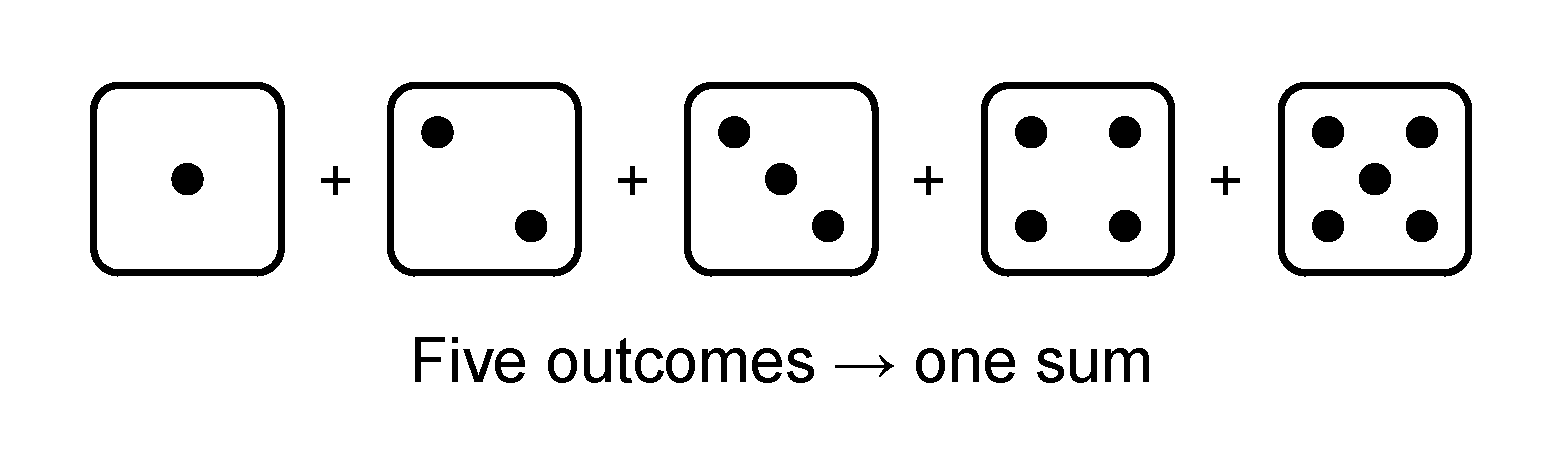
\includegraphics[width=\linewidth,height=.62\textheight,keepaspectratio]{asset-4bc7df832cfc39728ae98c671b6e9ecc1f50b3944e6c17a1bae41cc0f3da2f39.pdf}\end{center}

\medskip

A model expectation combines possible outcomes with their probabilities (\hyperref[material-5eae1c634cb6612f691623f47b0cc46cbd85ae3fd6b85b8e48bcd547c62df50b]{Eq.~\ref*{material-5eae1c634cb6612f691623f47b0cc46cbd85ae3fd6b85b8e48bcd547c62df50b}}). For one fair die the expected face value is 3.5 (\hyperref[material-3e77aacad0552fda4edca9ac9956e5ef4eb4d25ad9d58a459c2c0f4e0ad337b1]{Eq.~\ref*{material-3e77aacad0552fda4edca9ac9956e5ef4eb4d25ad9d58a459c2c0f4e0ad337b1}}). Adding the expectations of five dice gives an expected sum of 17.5 (\hyperref[material-7f50410fefd392ce399defabed85533811ddf093a5be5d3c9fc5a03eb7918871]{Eq.~\ref*{material-7f50410fefd392ce399defabed85533811ddf093a5be5d3c9fc5a03eb7918871}}). These values describe the probability model. An observed average summarizes the particular outcomes that were obtained.


\par\medskip
\noindent\begin{minipage}{\linewidth}
\refstepcounter{equation}\label{material-5eae1c634cb6612f691623f47b0cc46cbd85ae3fd6b85b8e48bcd547c62df50b}
\noindent\textbf{Eq.~\ref*{material-5eae1c634cb6612f691623f47b0cc46cbd85ae3fd6b85b8e48bcd547c62df50b}.} Discrete expectation as a probability-weighted sum, including all symbol and probability conventions.\par\nopagebreak
\begin{center}\begin{adjustbox}{max width=\linewidth}$\displaystyle \operatorname{E}[X] = \sum_{x \in \mathcal{S}} x\,P(X=x)$\end{adjustbox}\end{center}

\par\noindent\textbf{Symbols}

\par\noindent\textbf{X, E[X]} Discrete random variable and its distribution expectation.

\par\noindent\textbf{x, S} x is one possible numerical value of X; S is the set of all possible values.

\par\noindent\textbf{P(X=x)} Probability that X takes the value x. These model probabilities sum to 1 and weight the possible values; they are not observed sample frequencies.

\end{minipage}\par
\medskip

\par\medskip
\noindent\begin{minipage}{\linewidth}
\refstepcounter{equation}\label{material-3e77aacad0552fda4edca9ac9956e5ef4eb4d25ad9d58a459c2c0f4e0ad337b1}
\noindent\textbf{Eq.~\ref*{material-3e77aacad0552fda4edca9ac9956e5ef4eb4d25ad9d58a459c2c0f4e0ad337b1}.} Fair-die expectation: the six equally probable faces give 3.5.\par\nopagebreak
\begin{center}\begin{adjustbox}{max width=\linewidth}$\displaystyle \begin{aligned}\operatorname{E}[D]&=\frac{1+2+3+4+5+6}{6}\\&=3.5\end{aligned}$\end{adjustbox}\end{center}

\par\noindent\textbf{Symbols}

\par\noindent\textbf{D, E[D]} One fair die outcome and its expected value.

\par\noindent\textbf{1\ensuremath{\ldots}6, 1/6} Six faces, each with probability one sixth.

\end{minipage}\par
\medskip

\par\medskip
\noindent\begin{minipage}{\linewidth}
\refstepcounter{equation}\label{material-7f50410fefd392ce399defabed85533811ddf093a5be5d3c9fc5a03eb7918871}
\noindent\textbf{Eq.~\ref*{material-7f50410fefd392ce399defabed85533811ddf093a5be5d3c9fc5a03eb7918871}.} Expected sum of five fair dice: five times 3.5 gives 17.5.\par\nopagebreak
\begin{center}\begin{adjustbox}{max width=\linewidth}$\displaystyle \begin{aligned}S&=D_1+\cdots+D_5\\\operatorname{E}[S]&=5\times3.5=17.5\end{aligned}$\end{adjustbox}\end{center}

\par\noindent\textbf{Symbols}

\par\noindent\textbf{D\ensuremath{{}_j}, S} Outcome of die j; S is the sum of five outcomes.

\par\noindent\textbf{E[S], 3.5} Expected sum; each fair die has expectation 3.5.

\end{minipage}\par
\medskip

Repeating an independent experiment more often improves the stability of its average under the assumptions of the law of large numbers. The optional calculation in \hyperref[material-e19ca0a2d1200e7ed2e9f51375b680185cf799556d6bfe7d6d537feb3a627542]{Listing~\ref*{material-e19ca0a2d1200e7ed2e9f51375b680185cf799556d6bfe7d6d537feb3a627542}} compares averages based on different numbers of five-dice experiments. Individual sums continue to vary; increasing the number of experiments supplies more information about their common expectation. This distinction becomes essential when we later separate variation of individual measurements from variation of their average.


\par\medskip
\Needspace{8\baselineskip}
\refstepcounter{listing}\label{material-e19ca0a2d1200e7ed2e9f51375b680185cf799556d6bfe7d6d537feb3a627542}
\noindent\textbf{Listing~\ref*{material-e19ca0a2d1200e7ed2e9f51375b680185cf799556d6bfe7d6d537feb3a627542}.} Optional fixed-seed R comparison of averages from 5, 50 and 50,000 repeated five-dice experiments.\par\nopagebreak
\begin{Verbatim}[fontsize=\footnotesize,breaklines=true,breakanywhere=true]
set.seed(42)
sums <- replicate(50000, sum(sample(1:6, 5, replace = TRUE)))
n <- c(5, 50, 50000)
data.frame(n, mean = sapply(n, function(k) mean(sums[seq_len(k)])))
\end{Verbatim}

\par\noindent\textbf{set.seed(seed)}

Fixes the pseudorandom sequence for reproducible comparisons.

\par\noindent\textbf{replicate(n, expr)}

Repeats the five-dice experiment 50,000 times.

\par\noindent\textbf{sample(x, size, replace)}

Draws five fair-die outcomes for each experiment.

\par\noindent\textbf{sum(x)}

Adds the five outcomes in each repeated experiment.

\par\noindent\textbf{data.frame(...)}

Combines the repetition counts and their calculated averages as columns.

\par\noindent\textbf{sapply(x, function)}

Applies the supplied calculation to each repetition count.

\par\noindent\textbf{function(k)}

Defines a small calculation that receives one repetition count k.

\par\noindent\textbf{seq\_len(k)}

Creates indices 1 through k to select the first k available experiment sums.

\par\noindent\textbf{mean(x)}

Calculates the arithmetic mean of the selected experiment sums.

\par\noindent\textbf{c(...)}

Combines the three repetition counts into one vector.

\medskip

\clearpage
\section{The arithmetic mean preserves an additive total}
For equally weighted observations of an additive quantity, the arithmetic mean divides the observed total equally among the observations. Its definition in \hyperref[material-c0131e65df621d3d1dee13bdf8fefc08b4dc1e45608794f64c058b9855cb5466]{Eq.~\ref*{material-c0131e65df621d3d1dee13bdf8fefc08b4dc1e45608794f64c058b9855cb5466}} expresses that conservation of the total. The worked dice calculation in \hyperref[material-220b21265767036f251ea3f1bc4a3b6df88259d5ec843c4c86aa253c8ff96fc1]{Eq.~\ref*{material-220b21265767036f251ea3f1bc4a3b6df88259d5ec843c4c86aa253c8ff96fc1}} connects the general rule with a finite observed set; \hyperref[material-86173f0cd8562828fcd7487dc5da60122cd6cff59b8a5efc1553e3dfa11ae3b0]{Listing~\ref*{material-86173f0cd8562828fcd7487dc5da60122cd6cff59b8a5efc1553e3dfa11ae3b0}} supplies the optional executable example.


\par\medskip
\noindent\begin{minipage}{\linewidth}
\refstepcounter{equation}\label{material-c0131e65df621d3d1dee13bdf8fefc08b4dc1e45608794f64c058b9855cb5466}
\noindent\textbf{Eq.~\ref*{material-c0131e65df621d3d1dee13bdf8fefc08b4dc1e45608794f64c058b9855cb5466}.} Arithmetic mean of equally weighted observations, with the sample-size and unit conventions.\par\nopagebreak
\begin{center}\begin{adjustbox}{max width=\linewidth}$\displaystyle \bar{x} = \frac{1}{n} \sum_{i=1}^{n} x_i$\end{adjustbox}\end{center}

\par\noindent\textbf{Symbols}

\par\noindent\textbf{\ensuremath{\bar{x}}, x\ensuremath{{}_i}} Arithmetic sample mean and observation i, in the same unit.

\par\noindent\textbf{n, i, \ensuremath{\Sigma}} Sample size, observation index and sum over equally weighted numerical observations with meaningful addition. Normality is not required.

\end{minipage}\par
\medskip

\par\medskip
\noindent\begin{minipage}{\linewidth}
\refstepcounter{equation}\label{material-220b21265767036f251ea3f1bc4a3b6df88259d5ec843c4c86aa253c8ff96fc1}
\noindent\textbf{Eq.~\ref*{material-220b21265767036f251ea3f1bc4a3b6df88259d5ec843c4c86aa253c8ff96fc1}.} Worked arithmetic average of the authored dice results.\par\nopagebreak
\begin{center}\begin{adjustbox}{max width=\linewidth}$\displaystyle \begin{aligned}\bar{x}&=\frac{\sum_{i=1}^{n}x_i}{n}\\&=\frac{10+13+18+10+23}{5}\\&=\frac{74}{5}=14.8\end{aligned}$\end{adjustbox}\end{center}

\par\noindent\textbf{Symbols}

\par\noindent\textbf{\ensuremath{\bar{x}}, x\ensuremath{{}_i}} \ensuremath{\bar{x}} is the sample average of experiment sums; x\ensuremath{{}_i} is the observed five-dice sum from experiment i.

\par\noindent\textbf{n, i, \ensuremath{\Sigma}} Five equally weighted experiments; i indexes them; \ensuremath{\Sigma} adds their sums.

\end{minipage}\par
\medskip

\par\medskip
\Needspace{8\baselineskip}
\refstepcounter{listing}\label{material-86173f0cd8562828fcd7487dc5da60122cd6cff59b8a5efc1553e3dfa11ae3b0}
\noindent\textbf{Listing~\ref*{material-86173f0cd8562828fcd7487dc5da60122cd6cff59b8a5efc1553e3dfa11ae3b0}.} Optional R source for arithmetic averages of repeated dice experiments.\par\nopagebreak
\begin{Verbatim}[fontsize=\footnotesize,breaklines=true,breakanywhere=true]
set.seed(42)
sums <- replicate(5, sum(sample(1:6, 5, replace = TRUE)))
list(sums = sums, mean = mean(sums))
\end{Verbatim}

\par\noindent\textbf{set.seed(seed)}

Makes the pseudorandom draws reproducible.

\par\noindent\textbf{replicate(n, expr)}

Evaluates expr n times and collects each experiment sum.

\par\noindent\textbf{sample(x, size, replace)}

Draws five die faces from 1:6 with replacement.

\par\noindent\textbf{sum(x)}

Adds the five faces within one experiment.

\par\noindent\textbf{mean(x)}

Calculates the arithmetic mean of the five experiment sums.

\par\noindent\textbf{list(...)}

Returns the named sums and their mean together.

\medskip

The water measurements in \hyperref[material-47985308a110207e09fa3a9e1fb3c552daf3548ba5f591bbc57ca9927050d9cd]{Table~\ref*{material-47985308a110207e09fa3a9e1fb3c552daf3548ba5f591bbc57ca9927050d9cd}} transfer this reasoning to analytical concentrations. Each recorded value retains its unit and observation identity. If the observations have the same scientific role and equal weights, their arithmetic mean summarizes their concentration level. Pooling physical samples with different volumes instead calls for weights that represent those volumes, because the chemical total being conserved is analyte amount.


\par\medskip
\Needspace{8\baselineskip}
\refstepcounter{scripttable}\label{material-47985308a110207e09fa3a9e1fb3c552daf3548ba5f591bbc57ca9927050d9cd}
\noindent\textbf{Table~\ref*{material-47985308a110207e09fa3a9e1fb3c552daf3548ba5f591bbc57ca9927050d9cd}.} Authored water measurements used for the arithmetic-mean example, with their concentration units.\par\nopagebreak
\begin{longtable}{@{}p{\dimexpr0.250000\linewidth-2\tabcolsep\relax}p{\dimexpr0.250000\linewidth-2\tabcolsep\relax}p{\dimexpr0.250000\linewidth-2\tabcolsep\relax}p{\dimexpr0.250000\linewidth-2\tabcolsep\relax}@{}}
Observation & Oxygen & Nitrate & Iron \\ \hline
\endhead
1 & 8.5 & 3.2 & 5.2 \\ \hline
2 & 8.7 & 3.5 & 4.8 \\ \hline
3 & 8.6 & 3.3 & 5.1 \\ \hline
4 & 8.4 & 3.4 & 5.0 \\ \hline
5 & 8.8 & 3.6 & 4.9 \\ \hline
\end{longtable}
\medskip

The optional calculation in \hyperref[material-6ff7be4d519341c1a7638ce334764a848ccb3365aea0de27034ec3e9cacd5eec]{Listing~\ref*{material-6ff7be4d519341c1a7638ce334764a848ccb3365aea0de27034ec3e9cacd5eec}} reproduces the authored water example. Before using its result, state what the observations represent and why equal weighting is appropriate. The same numerical operation can summarize repeated readings, independent sample preparations or distinct water collections, but each design gives the resulting mean a different scope.


\par\medskip
\Needspace{8\baselineskip}
\refstepcounter{listing}\label{material-6ff7be4d519341c1a7638ce334764a848ccb3365aea0de27034ec3e9cacd5eec}
\noindent\textbf{Listing~\ref*{material-6ff7be4d519341c1a7638ce334764a848ccb3365aea0de27034ec3e9cacd5eec}.} Optional R reproduction of the water-concentration summary.\par\nopagebreak
\begin{Verbatim}[fontsize=\footnotesize,breaklines=true,breakanywhere=true]
fe <- c(5.2, 4.8, 5.1, 5.0, 4.9)
mean(fe)
\end{Verbatim}

\par\noindent\textbf{c(...)}

Combines the five measured concentrations into a vector.

\par\noindent\textbf{mean(x)}

Calculates the arithmetic mean of the five concentrations.

\medskip

The replicate measurements in \hyperref[material-8a02508feb566e286c4d87e0a986122952ae12f569b12e0a6d16190f527f4642]{Fig.~\ref*{material-8a02508feb566e286c4d87e0a986122952ae12f569b12e0a6d16190f527f4642}} and sensor readings in \hyperref[material-ea61b90ef1ea1eda78bf66e33887aa4b12fbfffe6f7f1c2cac25d21b89ffc93c]{Fig.~\ref*{material-ea61b90ef1ea1eda78bf66e33887aa4b12fbfffe6f7f1c2cac25d21b89ffc93c}} invite this design check. Combining sensor outputs requires comparable calibration; an uncertainty calculation additionally accounts for shared and independent errors. The simultaneous loads in \hyperref[material-0e3c947eea13dacfdfc8e271aa6ceb1a12857863ec64f2e8b81144428f9d7a2c]{Fig.~\ref*{material-0e3c947eea13dacfdfc8e271aa6ceb1a12857863ec64f2e8b81144428f9d7a2c}} instead contribute separate amounts to one total. Their sum describes the combined phosphorus input, while their arithmetic mean describes the average input per stream.


\par\medskip
\Needspace{10cm}
\refstepcounter{figure}\label{material-8a02508feb566e286c4d87e0a986122952ae12f569b12e0a6d16190f527f4642}
\noindent\textbf{Fig.~\ref*{material-8a02508feb566e286c4d87e0a986122952ae12f569b12e0a6d16190f527f4642}.} Three comparable nitrate replicate measurements: 4.8, 5.0 and 5.2 mg/L, with arithmetic mean 5.0 mg/L.\par\nopagebreak
\begin{center}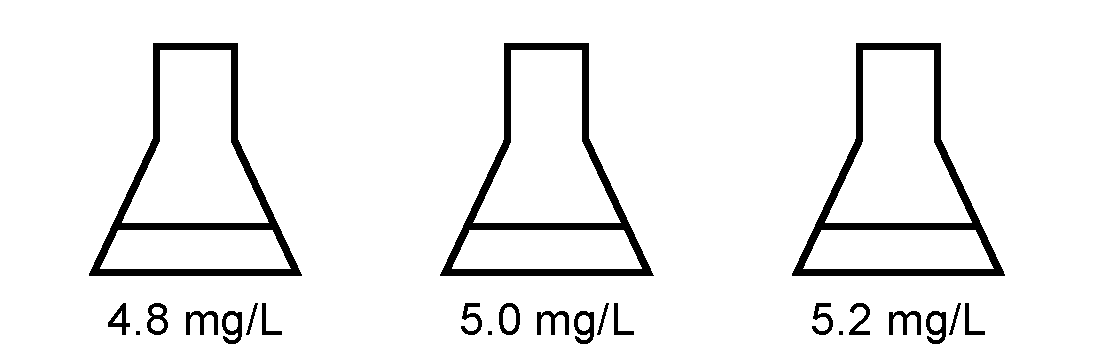
\includegraphics[width=\linewidth,height=.62\textheight,keepaspectratio]{asset-8dce1c57890e0912db2826a49e1e34b08b201198831c324a4bf67bbd3460fd97.pdf}\end{center}

\medskip

\par\medskip
\Needspace{10cm}
\refstepcounter{figure}\label{material-ea61b90ef1ea1eda78bf66e33887aa4b12fbfffe6f7f1c2cac25d21b89ffc93c}
\noindent\textbf{Fig.~\ref*{material-ea61b90ef1ea1eda78bf66e33887aa4b12fbfffe6f7f1c2cac25d21b89ffc93c}.} Three conductivity readings of 480, 500 and 520 µS/cm, with arithmetic mean 500 µS/cm.\par\nopagebreak
\begin{center}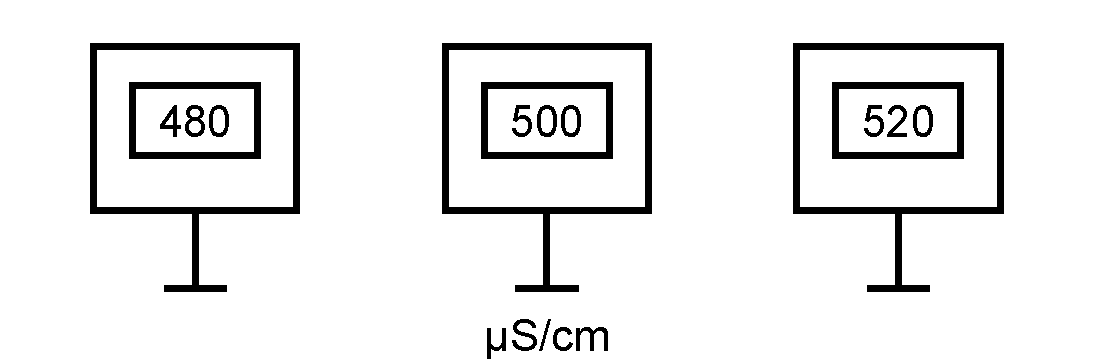
\includegraphics[width=\linewidth,height=.62\textheight,keepaspectratio]{asset-c0e17917a9b65e256b4a3bc6d32903ac4fdc314d952c6e435ad4cb821dcd0a6f.pdf}\end{center}

\medskip

\par\medskip
\Needspace{10cm}
\refstepcounter{figure}\label{material-0e3c947eea13dacfdfc8e271aa6ceb1a12857863ec64f2e8b81144428f9d7a2c}
\noindent\textbf{Fig.~\ref*{material-0e3c947eea13dacfdfc8e271aa6ceb1a12857863ec64f2e8b81144428f9d7a2c}.} Three simultaneous phosphorus inputs of 200, 300 and 200 g/s contribute a total of 700 g/s.\par\nopagebreak
\begin{center}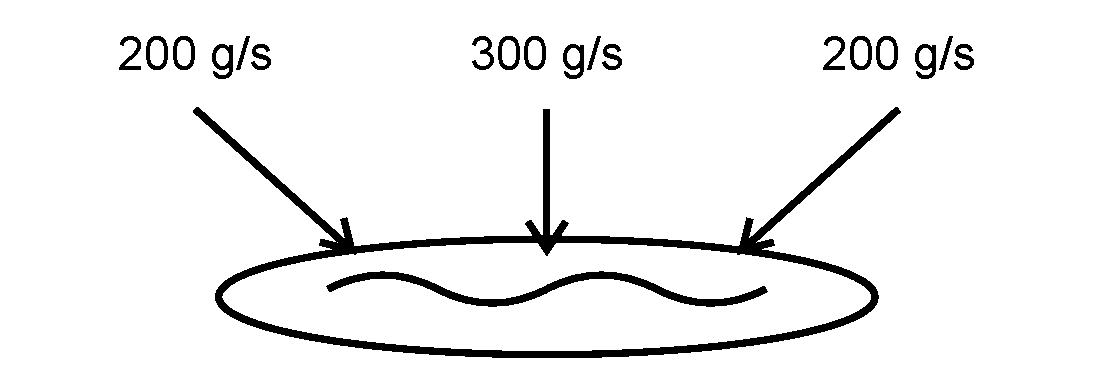
\includegraphics[width=\linewidth,height=.62\textheight,keepaspectratio]{asset-b685db1e67e68267fa87f9ca8b08d41e61fbbf6ffcde07a99706499908835493.pdf}\end{center}

\medskip

\clearpage
\section{The geometric mean preserves a product of positive factors}
Successive growth factors combine by multiplication. The process in \hyperref[material-5e68a098d3e93be9b7b9e807e6e0d59ee286fef3a12ccf9f0bebd49cc9881651]{Fig.~\ref*{material-5e68a098d3e93be9b7b9e807e6e0d59ee286fef3a12ccf9f0bebd49cc9881651}} therefore asks for a constant factor that reproduces the final product over the same number of steps. The arithmetic comparison in \hyperref[material-0711bca2cb3902976448ac820cce8500f78befd4957077589d1b396393dd5d09]{Eq.~\ref*{material-0711bca2cb3902976448ac820cce8500f78befd4957077589d1b396393dd5d09}} answers a sum-preservation question; the geometric mean in \hyperref[material-d094c81908c66b8d2e1fbba4960976a053b537c5049515f596d0e86ff68fff35]{Eq.~\ref*{material-d094c81908c66b8d2e1fbba4960976a053b537c5049515f596d0e86ff68fff35}} answers the product-preservation question posed by growth.


\par\medskip
\Needspace{10cm}
\refstepcounter{figure}\label{material-5e68a098d3e93be9b7b9e807e6e0d59ee286fef3a12ccf9f0bebd49cc9881651}
\noindent\textbf{Fig.~\ref*{material-5e68a098d3e93be9b7b9e807e6e0d59ee286fef3a12ccf9f0bebd49cc9881651}.} Successive growth stages combine through their multiplicative factors.\par\nopagebreak
\par\medskip\noindent\textcolor{pcd1}{\textbf{1. 100 CELLS}}\par
Start

\par\noindent $\longrightarrow$ 2. \ensuremath{\times} 2
\par\medskip\noindent\textcolor{pcd2}{\textbf{2. 200 CELLS}}\par
After period 1

\par\noindent $\longrightarrow$ 3. \ensuremath{\times} 8
\par\medskip\noindent\textcolor{pcd3}{\textbf{3. 1600 CELLS}}\par
After period 2


\medskip

\par\medskip
\noindent\begin{minipage}{\linewidth}
\refstepcounter{equation}\label{material-0711bca2cb3902976448ac820cce8500f78befd4957077589d1b396393dd5d09}
\noindent\textbf{Eq.~\ref*{material-0711bca2cb3902976448ac820cce8500f78befd4957077589d1b396393dd5d09}.} Arithmetic comparison for the authored growth factors.\par\nopagebreak
\begin{center}\begin{adjustbox}{max width=\linewidth}$\displaystyle \begin{aligned}A&=(2+8)/2=5\\100\times5^2&=2500\ne100\times2\times8=1600\end{aligned}$\end{adjustbox}\end{center}

\par\noindent\textbf{Symbols}

\par\noindent\textbf{A} Arithmetic average of growth factors 2 and 8: A = 5.

\par\noindent\textbf{100, 2} Initial count 100; exponent 2 applies one factor over two equal periods.

\end{minipage}\par
\medskip

\par\medskip
\noindent\begin{minipage}{\linewidth}
\refstepcounter{equation}\label{material-d094c81908c66b8d2e1fbba4960976a053b537c5049515f596d0e86ff68fff35}
\noindent\textbf{Eq.~\ref*{material-d094c81908c66b8d2e1fbba4960976a053b537c5049515f596d0e86ff68fff35}.} Geometric mean of positive values as a product-preserving constant factor.\par\nopagebreak
\begin{center}\begin{adjustbox}{max width=\linewidth}$\displaystyle G = \left(\prod_{i=1}^{n} x_i\right)^{1/n}, \qquad x_i > 0$\end{adjustbox}\end{center}

\par\noindent\textbf{Symbols}

\par\noindent\textbf{G, x\ensuremath{{}_i}} Geometric mean and positive input i.

\par\noindent\textbf{n, i, Π} Number of inputs, index and product over the inputs.

\end{minipage}\par
\medskip

The worked result in \hyperref[material-d0f583a42299f569e48655e2ac65f452bcf01becf9fa7dbca077ba7071f5adc3]{Eq.~\ref*{material-d0f583a42299f569e48655e2ac65f452bcf01becf9fa7dbca077ba7071f5adc3}} gives the equivalent constant growth factor for the authored sequence. Taking logarithms turns products of positive factors into sums, which explains the log-scale formulation in \hyperref[material-fe480c03581614cc7bed435dfa9dd55d635ebe6369b39fcaf51002c827ff8077]{Eq.~\ref*{material-fe480c03581614cc7bed435dfa9dd55d635ebe6369b39fcaf51002c827ff8077}}. Positivity is part of this real-valued logarithmic construction. The optional R source in \hyperref[material-5ea4a7a6f2710c94833962d59127cc7e971f5af284cc92def2030b2f16f80afe]{Listing~\ref*{material-5ea4a7a6f2710c94833962d59127cc7e971f5af284cc92def2030b2f16f80afe}} reproduces both the factors and their summaries.


\par\medskip
\noindent\begin{minipage}{\linewidth}
\refstepcounter{equation}\label{material-d0f583a42299f569e48655e2ac65f452bcf01becf9fa7dbca077ba7071f5adc3}
\noindent\textbf{Eq.~\ref*{material-d0f583a42299f569e48655e2ac65f452bcf01becf9fa7dbca077ba7071f5adc3}.} Worked geometric growth factor for the authored sequence.\par\nopagebreak
\begin{center}\begin{adjustbox}{max width=\linewidth}$\displaystyle \begin{aligned}G&=\sqrt{2\times8}=4\\100\times4^2&=1600=100\times2\times8\end{aligned}$\end{adjustbox}\end{center}

\par\noindent\textbf{Symbols}

\par\noindent\textbf{G} Equivalent factor 4 per equal period preserves the product 2 \ensuremath{\times} 8.

\par\noindent\textbf{100, 2} Initial count 100; two equal periods lead to 1600 cells.

\end{minipage}\par
\medskip

\par\medskip
\noindent\begin{minipage}{\linewidth}
\refstepcounter{equation}\label{material-fe480c03581614cc7bed435dfa9dd55d635ebe6369b39fcaf51002c827ff8077}
\noindent\textbf{Eq.~\ref*{material-fe480c03581614cc7bed435dfa9dd55d635ebe6369b39fcaf51002c827ff8077}.} Logarithmic formulation of the geometric mean, with its positive-domain and logarithm conventions.\par\nopagebreak
\begin{center}\begin{adjustbox}{max width=\linewidth}$\displaystyle G = \exp\left(\frac{1}{n}\sum_{i=1}^{n}\ln x_i\right), \qquad x_i > 0$\end{adjustbox}\end{center}

\par\noindent\textbf{Symbols}

\par\noindent\textbf{G, x\ensuremath{{}_i}} Geometric mean and positive input i.

\par\noindent\textbf{n, ln, exp} Number of inputs, natural logarithm and inverse exponential.

\end{minipage}\par
\medskip

\par\medskip
\Needspace{8\baselineskip}
\refstepcounter{listing}\label{material-5ea4a7a6f2710c94833962d59127cc7e971f5af284cc92def2030b2f16f80afe}
\noindent\textbf{Listing~\ref*{material-5ea4a7a6f2710c94833962d59127cc7e971f5af284cc92def2030b2f16f80afe}.} Optional R reproduction of the growth-factor comparison.\par\nopagebreak
\begin{Verbatim}[fontsize=\footnotesize,breaklines=true,breakanywhere=true]
factors <- c(2, 8)
g <- prod(factors)^(1 / length(factors))
list(geometric = g, final_cells = 100 * g^length(factors))
\end{Verbatim}

\par\noindent\textbf{c(...)}

Combines the two positive growth factors into a vector.

\par\noindent\textbf{prod(x)}

Multiplies the factors to obtain their total multiplier.

\par\noindent\textbf{length(x)}

Counts the factors, here the two equal-duration periods.

\par\noindent\textbf{list(...)}

Returns the geometric factor and reconstructed final count together.

\medskip

The microbial examples (\hyperref[material-99c28f8e994fbc24d0859fd9e4f27687afa5ab9c3cb0813c05219d0e5ee16e7d]{Eq.~\ref*{material-99c28f8e994fbc24d0859fd9e4f27687afa5ab9c3cb0813c05219d0e5ee16e7d}}, \hyperref[material-6b085c4776dfc4d690e310ba100f938f109c5b7c0ba4664f03a92ff3adaaffee]{Eq.~\ref*{material-6b085c4776dfc4d690e310ba100f938f109c5b7c0ba4664f03a92ff3adaaffee}}) and ratio examples (\hyperref[material-3d3233600dcb1c3956bee63b2ddcda699b9ebea623625da31787fee8d9d650ac]{Eq.~\ref*{material-3d3233600dcb1c3956bee63b2ddcda699b9ebea623625da31787fee8d9d650ac}}, \hyperref[material-66222a22efe87ed99c9d65b4efef6b6e837efd39e04416793b3d14b7adb2f734]{Eq.~\ref*{material-66222a22efe87ed99c9d65b4efef6b6e837efd39e04416793b3d14b7adb2f734}}) make the choice consequential. An arithmetic summary concerns the level on the original additive scale; a geometric summary concerns the level on the logarithmic scale or an equivalent multiplicative factor. State the intended meaning before selecting a summary, and preserve the measurement units or dimensionless ratio convention in the report.


\par\medskip
\noindent\begin{minipage}{\linewidth}
\refstepcounter{equation}\label{material-99c28f8e994fbc24d0859fd9e4f27687afa5ab9c3cb0813c05219d0e5ee16e7d}
\noindent\textbf{Eq.~\ref*{material-99c28f8e994fbc24d0859fd9e4f27687afa5ab9c3cb0813c05219d0e5ee16e7d}.} Arithmetic summary of the authored microbial measurements.\par\nopagebreak
\begin{center}\begin{adjustbox}{max width=\linewidth}$\displaystyle \begin{aligned}A&=\frac{10+100+10000}{3}\\&=3370\end{aligned}$\end{adjustbox}\end{center}

\par\noindent\textbf{Symbols}

\par\noindent\textbf{A} Arithmetic mean of the three equally weighted counts.

\par\noindent\textbf{10, 100, 10000} Illustrative counts per 100 mL; result has the same unit.

\end{minipage}\par
\medskip

\par\medskip
\noindent\begin{minipage}{\linewidth}
\refstepcounter{equation}\label{material-6b085c4776dfc4d690e310ba100f938f109c5b7c0ba4664f03a92ff3adaaffee}
\noindent\textbf{Eq.~\ref*{material-6b085c4776dfc4d690e310ba100f938f109c5b7c0ba4664f03a92ff3adaaffee}.} Geometric summary of the same positive microbial measurements.\par\nopagebreak
\begin{center}\begin{adjustbox}{max width=\linewidth}$\displaystyle \begin{aligned}G&=\sqrt[3]{10\times100\times10000}\\&\approx215.44\end{aligned}$\end{adjustbox}\end{center}

\par\noindent\textbf{Symbols}

\par\noindent\textbf{G, \ensuremath{\sqrt[3]{\vphantom{x}}}} Geometric mean of three positive counts; \ensuremath{\sqrt[3]{\vphantom{x}}} is the cube root.

\par\noindent\textbf{10, 100, 10000} Illustrative counts per 100 mL; result has the same unit.

\end{minipage}\par
\medskip

\par\medskip
\noindent\begin{minipage}{\linewidth}
\refstepcounter{equation}\label{material-3d3233600dcb1c3956bee63b2ddcda699b9ebea623625da31787fee8d9d650ac}
\noindent\textbf{Eq.~\ref*{material-3d3233600dcb1c3956bee63b2ddcda699b9ebea623625da31787fee8d9d650ac}.} Arithmetic summary of the authored dimensionless ratios.\par\nopagebreak
\begin{center}\begin{adjustbox}{max width=\linewidth}$\displaystyle A=(0.5+2+5)/3=2.5$\end{adjustbox}\end{center}

\par\noindent\textbf{Symbols}

\par\noindent\textbf{A} Arithmetic mean of three equally weighted ratios.

\par\noindent\textbf{0.5, 2, 5} Illustrative dimensionless ratios.

\end{minipage}\par
\medskip

\par\medskip
\noindent\begin{minipage}{\linewidth}
\refstepcounter{equation}\label{material-66222a22efe87ed99c9d65b4efef6b6e837efd39e04416793b3d14b7adb2f734}
\noindent\textbf{Eq.~\ref*{material-66222a22efe87ed99c9d65b4efef6b6e837efd39e04416793b3d14b7adb2f734}.} Geometric summary of the same dimensionless ratios.\par\nopagebreak
\begin{center}\begin{adjustbox}{max width=\linewidth}$\displaystyle G=\sqrt[3]{0.5\times2\times5}\approx1.710$\end{adjustbox}\end{center}

\par\noindent\textbf{Symbols}

\par\noindent\textbf{G, \ensuremath{\sqrt[3]{\vphantom{x}}}} Equivalent factor with equal logarithmic weight; cube root for three inputs.

\par\noindent\textbf{0.5, 2, 5} Positive dimensionless input ratios.

\end{minipage}\par
\medskip

The growth sketch in \hyperref[material-8dfbe34520537b724d09d74dfbbde56287f889bdbd40eb2e0bf303b1052b2971]{Fig.~\ref*{material-8dfbe34520537b724d09d74dfbbde56287f889bdbd40eb2e0bf303b1052b2971}} represents successive populations schematically. The microplastic and pesticide comparisons (\hyperref[material-9180347fc8238eaaa2890b4a6b4cfed914939b71950d48f1c529b7b19bdbf016]{Fig.~\ref*{material-9180347fc8238eaaa2890b4a6b4cfed914939b71950d48f1c529b7b19bdbf016}}, \hyperref[material-421f9a594ecf5325cbb0b26c4fa108e777b35e5ccbb29c3a5b199a838df97e85]{Fig.~\ref*{material-421f9a594ecf5325cbb0b26c4fa108e777b35e5ccbb29c3a5b199a838df97e85}}) instead contain separate positive sample values. A geometric mean can summarize their log-scale centre. Assigning a population distribution such as a Lognormal model is an additional modelling step that draws on sampling evidence and the measurement process.


\par\medskip
\Needspace{10cm}
\refstepcounter{figure}\label{material-8dfbe34520537b724d09d74dfbbde56287f889bdbd40eb2e0bf303b1052b2971}
\noindent\textbf{Fig.~\ref*{material-8dfbe34520537b724d09d74dfbbde56287f889bdbd40eb2e0bf303b1052b2971}.} Illustrative populations of 100, 200 and 1600 over equal periods correspond to successive factors 2 and 8.\par\nopagebreak
\begin{center}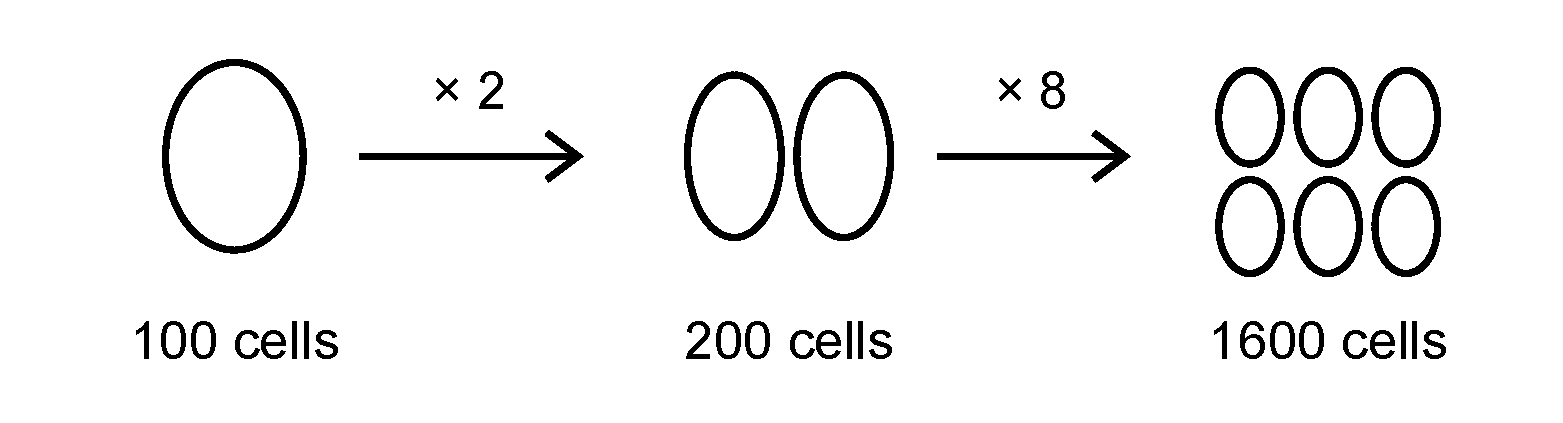
\includegraphics[width=\linewidth,height=.62\textheight,keepaspectratio]{asset-bdd291a999980ad19f69a64fa3dff019e3e8b3c4dd05b5796f49ea22d453dc29.pdf}\end{center}

\medskip

\par\medskip
\Needspace{10cm}
\refstepcounter{figure}\label{material-9180347fc8238eaaa2890b4a6b4cfed914939b71950d48f1c529b7b19bdbf016}
\noindent\textbf{Fig.~\ref*{material-9180347fc8238eaaa2890b4a6b4cfed914939b71950d48f1c529b7b19bdbf016}.} Separate samples containing 100, 1000 and 10000 particles/kg illustrate three multiplicative concentration levels.\par\nopagebreak
\begin{center}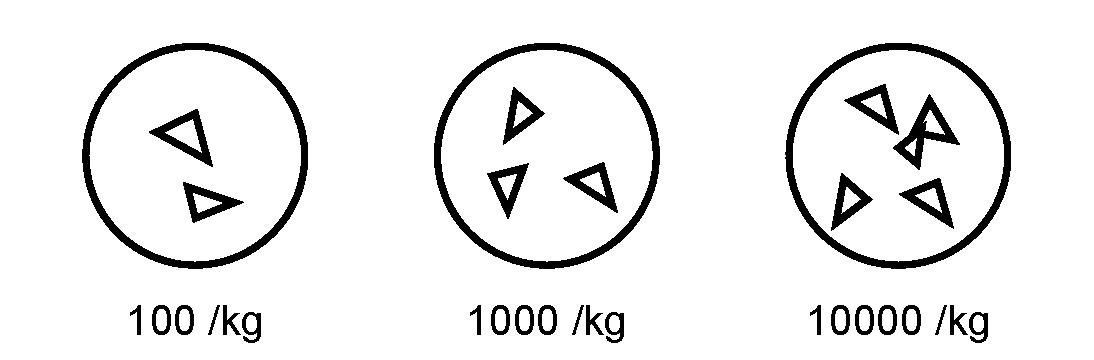
\includegraphics[width=\linewidth,height=.62\textheight,keepaspectratio]{asset-16f9a8312330caf14b40c7a606d82e3b99015a4690603573e7b9920ef1c8dda4.pdf}\end{center}

\medskip

\par\medskip
\Needspace{10cm}
\refstepcounter{figure}\label{material-421f9a594ecf5325cbb0b26c4fa108e777b35e5ccbb29c3a5b199a838df97e85}
\noindent\textbf{Fig.~\ref*{material-421f9a594ecf5325cbb0b26c4fa108e777b35e5ccbb29c3a5b199a838df97e85}.} Pesticide concentrations of 0.01, 0.1 and 1.0 µg/L at three sampling sites are successive tenfold levels.\par\nopagebreak
\begin{center}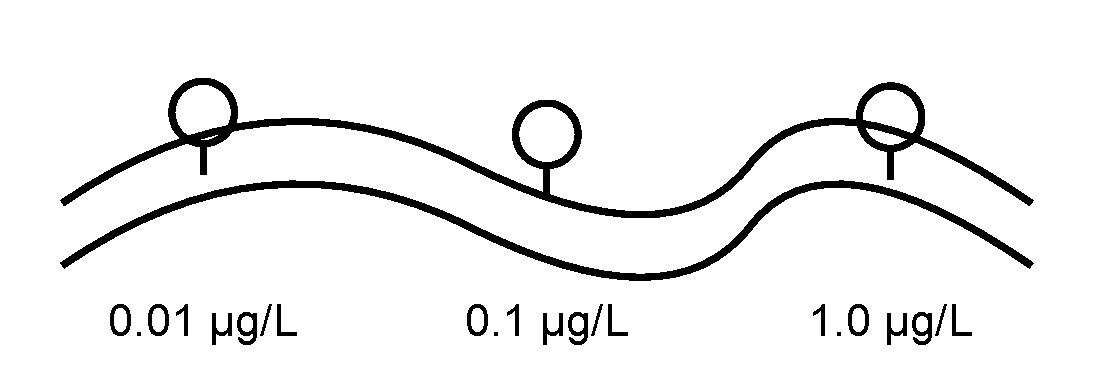
\includegraphics[width=\linewidth,height=.62\textheight,keepaspectratio]{asset-cbd8d43b40b391996033d89acf02428ed7298981b006c1e3750c0aec31811df9.pdf}\end{center}

\medskip

\clearpage
\section{Equal amounts make reciprocal rates the additive quantities}
A journey over equal distances provides a rate question with a clear conserved quantity. Total distance is the sum of the distances; total travel time is the sum of each distance divided by its speed. The arithmetic and geometric comparisons (\hyperref[material-7e1e47a2d055d93d2c2bb9e796a3d8daf806c98dcdebf992636e6e38a6193b00]{Eq.~\ref*{material-7e1e47a2d055d93d2c2bb9e796a3d8daf806c98dcdebf992636e6e38a6193b00}}, \hyperref[material-732e97361db28f7ebe1cfc3177f07c43fff17c21910ad178c159ee4f2bb71d85]{Eq.~\ref*{material-732e97361db28f7ebe1cfc3177f07c43fff17c21910ad178c159ee4f2bb71d85}}) motivate calculating the whole journey from these totals.


\par\medskip
\noindent\begin{minipage}{\linewidth}
\refstepcounter{equation}\label{material-7e1e47a2d055d93d2c2bb9e796a3d8daf806c98dcdebf992636e6e38a6193b00}
\noindent\textbf{Eq.~\ref*{material-7e1e47a2d055d93d2c2bb9e796a3d8daf806c98dcdebf992636e6e38a6193b00}.} Arithmetic comparison of the speeds in the equal-distance journey.\par\nopagebreak
\begin{center}\begin{adjustbox}{max width=\linewidth}$\displaystyle \begin{aligned}A&=(10+2)/2=6\;\mathrm{m/s}\\t_A&=200/6\approx33.33\;\mathrm{s}\end{aligned}$\end{adjustbox}\end{center}

\par\noindent\textbf{Symbols}

\par\noindent\textbf{A} Arithmetic average of the two speeds, in m/s.

\par\noindent\textbf{t\_A, 200 m} Predicted journey time if both 100 m sections were travelled at A.

\end{minipage}\par
\medskip

\par\medskip
\noindent\begin{minipage}{\linewidth}
\refstepcounter{equation}\label{material-732e97361db28f7ebe1cfc3177f07c43fff17c21910ad178c159ee4f2bb71d85}
\noindent\textbf{Eq.~\ref*{material-732e97361db28f7ebe1cfc3177f07c43fff17c21910ad178c159ee4f2bb71d85}.} Geometric comparison of the same journey speeds.\par\nopagebreak
\begin{center}\begin{adjustbox}{max width=\linewidth}$\displaystyle \begin{aligned}G&=\sqrt{10\times2}\approx4.472\;\mathrm{m/s}\\t_G&=200/\sqrt{20}\approx44.72\;\mathrm{s}\end{aligned}$\end{adjustbox}\end{center}

\par\noindent\textbf{Symbols}

\par\noindent\textbf{G} Geometric average of the two positive speeds, in m/s.

\par\noindent\textbf{t\_G, 200 m} Predicted journey time at constant speed G over the total distance.

\end{minipage}\par
\medskip

For equal distances and positive speeds, this calculation produces the harmonic mean (\hyperref[material-fa20634f2344b32b9494dfa5d924bcbfe7380937106fcf95aa1f7237bcddf7f9]{Eq.~\ref*{material-fa20634f2344b32b9494dfa5d924bcbfe7380937106fcf95aa1f7237bcddf7f9}}). The worked speed result in \hyperref[material-050414e88d5f317f964b774d41c2a8da50013081b126bf1cfc53704cf50bebeb]{Eq.~\ref*{material-050414e88d5f317f964b774d41c2a8da50013081b126bf1cfc53704cf50bebeb}} and total-time check in \hyperref[material-026ca5635c6acd8939776eb034177a4ebc97c9a3053ccdddc8f699e85cf8a32c]{Eq.~\ref*{material-026ca5635c6acd8939776eb034177a4ebc97c9a3053ccdddc8f699e85cf8a32c}} express the same journey in complementary ways. The optional source in \hyperref[material-0c21e0e247b013e8c3439f5fba965fa07b3ce765c81cb447959df3ce22d8d359]{Listing~\ref*{material-0c21e0e247b013e8c3439f5fba965fa07b3ce765c81cb447959df3ce22d8d359}} reproduces the calculation. Equal-duration segments instead give time weights, so the weighting follows the design of the journey.


\par\medskip
\noindent\begin{minipage}{\linewidth}
\refstepcounter{equation}\label{material-fa20634f2344b32b9494dfa5d924bcbfe7380937106fcf95aa1f7237bcddf7f9}
\noindent\textbf{Eq.~\ref*{material-fa20634f2344b32b9494dfa5d924bcbfe7380937106fcf95aa1f7237bcddf7f9}.} Harmonic mean of positive rates for equally weighted amounts.\par\nopagebreak
\begin{center}\begin{adjustbox}{max width=\linewidth}$\displaystyle H = \frac{n}{\sum_{i=1}^{n} 1/x_i}$\end{adjustbox}\end{center}

\par\noindent\textbf{Symbols}

\par\noindent\textbf{H, x\ensuremath{{}_i}} Harmonic mean and nonzero input i; rate examples use positive values.

\par\noindent\textbf{n, \ensuremath{\Sigma} 1/x\ensuremath{{}_i}} n counts the inputs; add their reciprocals. For speeds in m/s, 1/x\ensuremath{{}_i} is time per metre (s/m), so H is again in m/s.

\end{minipage}\par
\medskip

\par\medskip
\noindent\begin{minipage}{\linewidth}
\refstepcounter{equation}\label{material-050414e88d5f317f964b774d41c2a8da50013081b126bf1cfc53704cf50bebeb}
\noindent\textbf{Eq.~\ref*{material-050414e88d5f317f964b774d41c2a8da50013081b126bf1cfc53704cf50bebeb}.} Worked overall speed for the equal-distance journey.\par\nopagebreak
\begin{center}\begin{adjustbox}{max width=\linewidth}$\displaystyle \begin{aligned}v_H&=\frac{2}{1/10+1/2}\\&=\frac{10}{3}\;\mathrm{m/s}\\&\approx3.333\;\mathrm{m/s}\end{aligned}$\end{adjustbox}\end{center}

\par\noindent\textbf{Symbols}

\par\noindent\textbf{v\_H} Harmonic speed in m/s; use exact 10/3 for the next calculation.

\par\noindent\textbf{2, 10, 2} Two equal 100 m sections; positive speeds 10 and 2 m/s.

\end{minipage}\par
\medskip

\par\medskip
\noindent\begin{minipage}{\linewidth}
\refstepcounter{equation}\label{material-026ca5635c6acd8939776eb034177a4ebc97c9a3053ccdddc8f699e85cf8a32c}
\noindent\textbf{Eq.~\ref*{material-026ca5635c6acd8939776eb034177a4ebc97c9a3053ccdddc8f699e85cf8a32c}.} Total-distance divided by total-time check of the harmonic speed.\par\nopagebreak
\begin{center}\begin{adjustbox}{max width=\linewidth}$\displaystyle \begin{aligned}t&=\frac{d}{v_H}\\&=\frac{200}{10/3}\\&=60\;\mathrm{s}\end{aligned}$\end{adjustbox}\end{center}

\par\noindent\textbf{Symbols}

\par\noindent\textbf{t} Total journey time in seconds, not one section time.

\par\noindent\textbf{d, v\_H} Total distance 100 + 100 = 200 m; exact speed 10/3 m/s.

\end{minipage}\par
\medskip

\par\medskip
\Needspace{8\baselineskip}
\refstepcounter{listing}\label{material-0c21e0e247b013e8c3439f5fba965fa07b3ce765c81cb447959df3ce22d8d359}
\noindent\textbf{Listing~\ref*{material-0c21e0e247b013e8c3439f5fba965fa07b3ce765c81cb447959df3ce22d8d359}.} Optional R reproduction of the journey calculation.\par\nopagebreak
\begin{Verbatim}[fontsize=\footnotesize,breaklines=true,breakanywhere=true]
speeds <- c(10, 2)
distances <- rep(100, 2)
times <- distances / speeds
list(times_s = times, total_time_s = sum(times),
     overall_m_s = sum(distances) / sum(times),
     harmonic_m_s = 1 / mean(1 / speeds))
\end{Verbatim}

\par\noindent\textbf{c(...)}

Combines the two section speeds into a vector.

\par\noindent\textbf{rep(x, times)}

Repeats 100 m twice to represent equal section distances.

\par\noindent\textbf{sum(x)}

Adds section distances or travel times to their journey totals.

\par\noindent\textbf{mean(x)}

Averages reciprocal speeds; taking its reciprocal gives the harmonic mean.

\par\noindent\textbf{list(...)}

Returns named times and speeds together, with units in their names.

\medskip

Pumping equal volumes uses the same reciprocal-rate reasoning; \hyperref[material-fd9a2a32bcea0c48d41d5a5c9ffd9bb041bcd49eb81f6da55cf45ab6bf697a41]{Listing~\ref*{material-fd9a2a32bcea0c48d41d5a5c9ffd9bb041bcd49eb81f6da55cf45ab6bf697a41}} retains the executable practice example. Transport through equal-thickness layers supplies a second chemical application (\hyperref[material-69e7e5a9550aebfaa52f49f1ae1b908bc606648e2ac9cd574df907de3ef12b29]{Eq.~\ref*{material-69e7e5a9550aebfaa52f49f1ae1b908bc606648e2ac9cd574df907de3ef12b29}}, \hyperref[material-2a9abd14d1176d27ebf10dc55fd9776251e69c464a95b8ddd5403532fc184ca4]{Fig.~\ref*{material-2a9abd14d1176d27ebf10dc55fd9776251e69c464a95b8ddd5403532fc184ca4}}). Here resistances add in series under the authored steady-state assumptions, with common area, continuity of transport and the specified reaction and partition conditions. These physical assumptions determine when the harmonic construction describes the effective transport property.


\par\medskip
\Needspace{8\baselineskip}
\refstepcounter{listing}\label{material-fd9a2a32bcea0c48d41d5a5c9ffd9bb041bcd49eb81f6da55cf45ab6bf697a41}
\noindent\textbf{Listing~\ref*{material-fd9a2a32bcea0c48d41d5a5c9ffd9bb041bcd49eb81f6da55cf45ab6bf697a41}.} Optional R practice for successive equal-volume pumping batches.\par\nopagebreak
\begin{Verbatim}[fontsize=\footnotesize,breaklines=true,breakanywhere=true]
rates <- c(10, 2, 5)
volumes <- rep(10, 3)
times <- volumes / rates
list(times = times,
     overall = sum(volumes) / sum(times),
     harmonic = 1 / mean(1 / rates),
     arithmetic = mean(rates))
\end{Verbatim}

\par\noindent\textbf{c(...)}

Combines the three rates into a vector.

\par\noindent\textbf{rep(x, times)}

Repeats a batch volume three times, matching one batch to each rate.

\par\noindent\textbf{sum(x)}

Adds all batch volumes or all pumping times.

\par\noindent\textbf{mean(x)}

Calculates the arithmetic mean, here for comparison with overall rate.

\par\noindent\textbf{list(...)}

Returns the named times and rates together.

\medskip

\par\medskip
\noindent\begin{minipage}{\linewidth}
\refstepcounter{equation}\label{material-69e7e5a9550aebfaa52f49f1ae1b908bc606648e2ac9cd574df907de3ef12b29}
\noindent\textbf{Eq.~\ref*{material-69e7e5a9550aebfaa52f49f1ae1b908bc606648e2ac9cd574df907de3ef12b29}.} Effective transport through equal-thickness layers in series under the authored steady-state model.\par\nopagebreak
\begin{center}\begin{adjustbox}{max width=\linewidth}$\displaystyle D_{\mathrm{eff}}=\frac{2}{1/(2\times10^{-6})+1/(10^{-8})}\approx1.99\times10^{-8}\;\mathrm{m^2/s}$\end{adjustbox}\end{center}

\par\noindent\textbf{Symbols}

\par\noindent\textbf{D\ensuremath{{}_e}ff} Effective diffusion coefficient in m\ensuremath{{}^2}/s for two equal series layers.

\par\noindent\textbf{D\ensuremath{{}_1}, D\ensuremath{{}_2}} 2 \ensuremath{\times} 10\ensuremath{{}^-}\ensuremath{{}^6} and 10\ensuremath{{}^-}\ensuremath{{}^8} m\ensuremath{{}^2}/s; equal thickness/area, steady state, no reaction or partition jump.

\end{minipage}\par
\medskip

\par\medskip
\Needspace{10cm}
\refstepcounter{figure}\label{material-2a9abd14d1176d27ebf10dc55fd9776251e69c464a95b8ddd5403532fc184ca4}
\noindent\textbf{Fig.~\ref*{material-2a9abd14d1176d27ebf10dc55fd9776251e69c464a95b8ddd5403532fc184ca4}.} Layer sequence and transport context for the series-resistance calculation.\par\nopagebreak
\par\medskip\noindent\textcolor{pcd1}{\textbf{1. LAYER 1}}\par
D = 2 \ensuremath{\times} 10\textasciicircum{}-6 m\ensuremath{{}^2}/s
Thickness L, area A

\par\noindent $\longrightarrow$ 2. same steady flux
\par\medskip\noindent\textcolor{pcd2}{\textbf{2. LAYER 2}}\par
D = 10\textasciicircum{}-8 m\ensuremath{{}^2}/s
Thickness L, area A


\medskip

The journey and pumping sketches (\hyperref[material-4d177fcefed3503cb5d85c7fdd29f38fb1db23307414ca8f2237f34aa8418131]{Fig.~\ref*{material-4d177fcefed3503cb5d85c7fdd29f38fb1db23307414ca8f2237f34aa8418131}}, \hyperref[material-b9e76963ade8580810bbb078ba71df790ef973ee5ec331330fa9cbfb286e7a9e]{Fig.~\ref*{material-b9e76963ade8580810bbb078ba71df790ef973ee5ec331330fa9cbfb286e7a9e}}) retain the equal distances and equal volumes that justify the reciprocal weighting. The reactor sequence in \hyperref[material-4d56a55206805e774d2cd006d077955500aa391bba99f0afe2791ce1d15d0a82]{Fig.~\ref*{material-4d56a55206805e774d2cd006d077955500aa391bba99f0afe2791ce1d15d0a82}} poses a further modelling question. Deriving an effective reaction rate requires the reactor volumes, residence times and an appropriate kinetic and transport model. The ordering of the tanks supplies the process context; the physical model supplies the combination rule.


\par\medskip
\Needspace{10cm}
\refstepcounter{figure}\label{material-4d177fcefed3503cb5d85c7fdd29f38fb1db23307414ca8f2237f34aa8418131}
\noindent\textbf{Fig.~\ref*{material-4d177fcefed3503cb5d85c7fdd29f38fb1db23307414ca8f2237f34aa8418131}.} Two 100 m sections at 10 and 2 m/s take 10 and 50 seconds, giving 200 m in 60 seconds.\par\nopagebreak
\begin{center}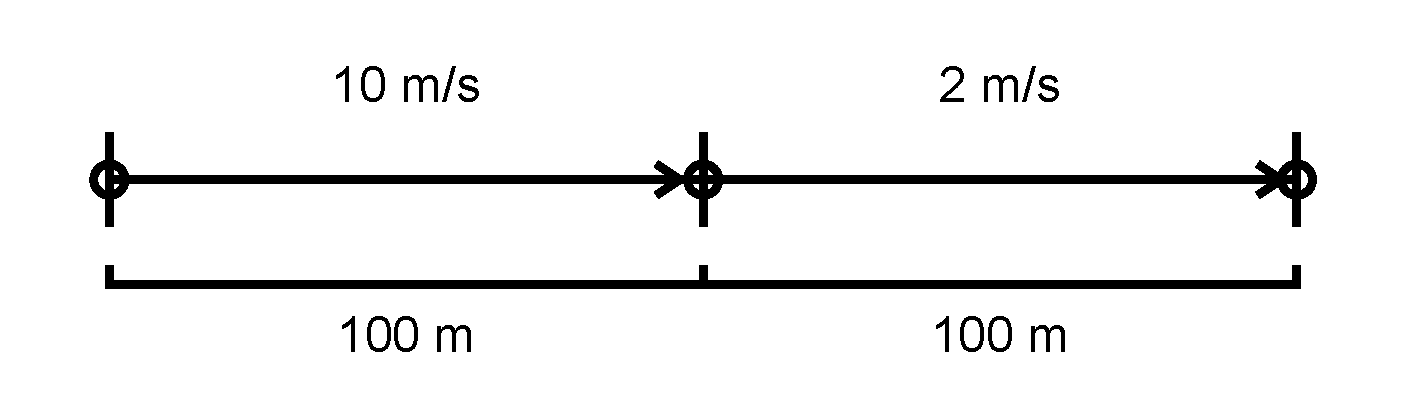
\includegraphics[width=\linewidth,height=.62\textheight,keepaspectratio]{asset-691652d98ccabe5ba0d0fc77c327022a3a1357aaff2550b9904772c86eeb0d94.pdf}\end{center}

\medskip

\par\medskip
\Needspace{10cm}
\refstepcounter{figure}\label{material-b9e76963ade8580810bbb078ba71df790ef973ee5ec331330fa9cbfb286e7a9e}
\noindent\textbf{Fig.~\ref*{material-b9e76963ade8580810bbb078ba71df790ef973ee5ec331330fa9cbfb286e7a9e}.} Three 10 L batches at 10, 2 and 5 L/min take 1, 5 and 2 minutes: 30 L in 8 minutes.\par\nopagebreak
\begin{center}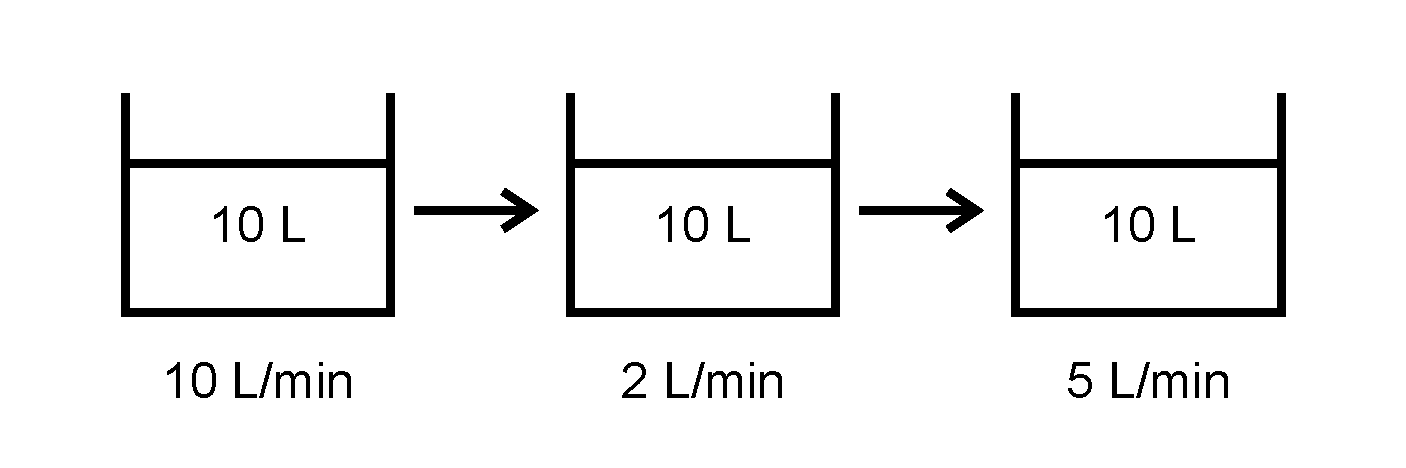
\includegraphics[width=\linewidth,height=.62\textheight,keepaspectratio]{asset-5084a27f6315169732ca579b4212ee1a1fd6463ac2149fb3ddd731410e0128cf.pdf}\end{center}

\medskip

\par\medskip
\Needspace{10cm}
\refstepcounter{figure}\label{material-4d56a55206805e774d2cd006d077955500aa391bba99f0afe2791ce1d15d0a82}
\noindent\textbf{Fig.~\ref*{material-4d56a55206805e774d2cd006d077955500aa391bba99f0afe2791ce1d15d0a82}.} Ordered reactor stages with rate constants 0.5, 1.0 and 2.0 per hour; the process model determines how their effects combine.\par\nopagebreak
\begin{center}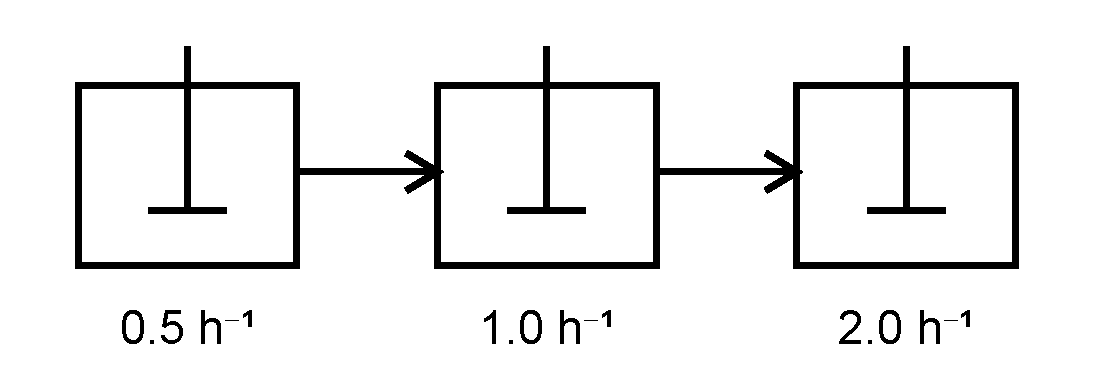
\includegraphics[width=\linewidth,height=.62\textheight,keepaspectratio]{asset-c06a25db4a769c87e0830bae3860ed18f813e3feb8b0f682ae08089200a179d6.pdf}\end{center}

\medskip

\clearpage
\section{The median locates the centre of the ordered observations}
A location summary can also be defined through rank. The turbidity example contains four observations around 2.0–2.3 NTU and an event at 45.0 NTU. Its arithmetic mean (\hyperref[material-1cc2b7e19b42d33b77bbe5ff429fa8931603285fc84cb1b6ac0a55350ee77182]{Eq.~\ref*{material-1cc2b7e19b42d33b77bbe5ff429fa8931603285fc84cb1b6ac0a55350ee77182}}) includes the magnitude of that event. The observation-order and sorted-order table in \hyperref[material-f8b733cd62f46b989d9d5d07ec5d16dadb8f91f5b7d5a3012e0958c289fb4ace]{Table~\ref*{material-f8b733cd62f46b989d9d5d07ec5d16dadb8f91f5b7d5a3012e0958c289fb4ace}} distinguishes the time sequence from the rank sequence, while \hyperref[material-c6635b0e3d3bd31a3209f9c84e047b609e4a0bfe537a44580ebcefacb4fa4ca0]{Fig.~\ref*{material-c6635b0e3d3bd31a3209f9c84e047b609e4a0bfe537a44580ebcefacb4fa4ca0}} retains the event in its observational context.


\par\medskip
\noindent\begin{minipage}{\linewidth}
\refstepcounter{equation}\label{material-1cc2b7e19b42d33b77bbe5ff429fa8931603285fc84cb1b6ac0a55350ee77182}
\noindent\textbf{Eq.~\ref*{material-1cc2b7e19b42d33b77bbe5ff429fa8931603285fc84cb1b6ac0a55350ee77182}.} Arithmetic mean of the five turbidity observations, including the 45.0 NTU event.\par\nopagebreak
\begin{center}\begin{adjustbox}{max width=\linewidth}$\displaystyle \bar{x}=\frac{53.6}{5}=10.72\;\mathrm{NTU}$\end{adjustbox}\end{center}

\par\noindent\textbf{Symbols}

\par\noindent\textbf{\ensuremath{\bar{x}}} Arithmetic mean of all five values, in NTU.

\par\noindent\textbf{53.6, 5} Sum 2.1 + 2.3 + 2.0 + 2.2 + 45.0; five equal weights.

\end{minipage}\par
\medskip

\par\medskip
\Needspace{8\baselineskip}
\refstepcounter{scripttable}\label{material-f8b733cd62f46b989d9d5d07ec5d16dadb8f91f5b7d5a3012e0958c289fb4ace}
\noindent\textbf{Table~\ref*{material-f8b733cd62f46b989d9d5d07ec5d16dadb8f91f5b7d5a3012e0958c289fb4ace}.} The same turbidity values in observation order and sorted order; day and rank are distinct indices.\par\nopagebreak
\begin{longtable}{@{}p{\dimexpr0.333333\linewidth-2\tabcolsep\relax}p{\dimexpr0.333333\linewidth-2\tabcolsep\relax}p{\dimexpr0.333333\linewidth-2\tabcolsep\relax}@{}}
Day / rank & Day order & Rank order \\ \hline
\endhead
1 & 2.1 & 2.0 \\ \hline
2 & 2.3 & 2.1 \\ \hline
3 & 2.0 & 2.2 \\ \hline
4 & 2.2 & 2.3 \\ \hline
5 & 45.0 & 45.0 \\ \hline
\end{longtable}
\medskip

\par\medskip
\Needspace{10cm}
\refstepcounter{figure}\label{material-c6635b0e3d3bd31a3209f9c84e047b609e4a0bfe537a44580ebcefacb4fa4ca0}
\noindent\textbf{Fig.~\ref*{material-c6635b0e3d3bd31a3209f9c84e047b609e4a0bfe537a44580ebcefacb4fa4ca0}.} Turbidity by observation day: the 45.0 NTU event remains visible alongside four values near 2 NTU.\par\nopagebreak
\begin{center}
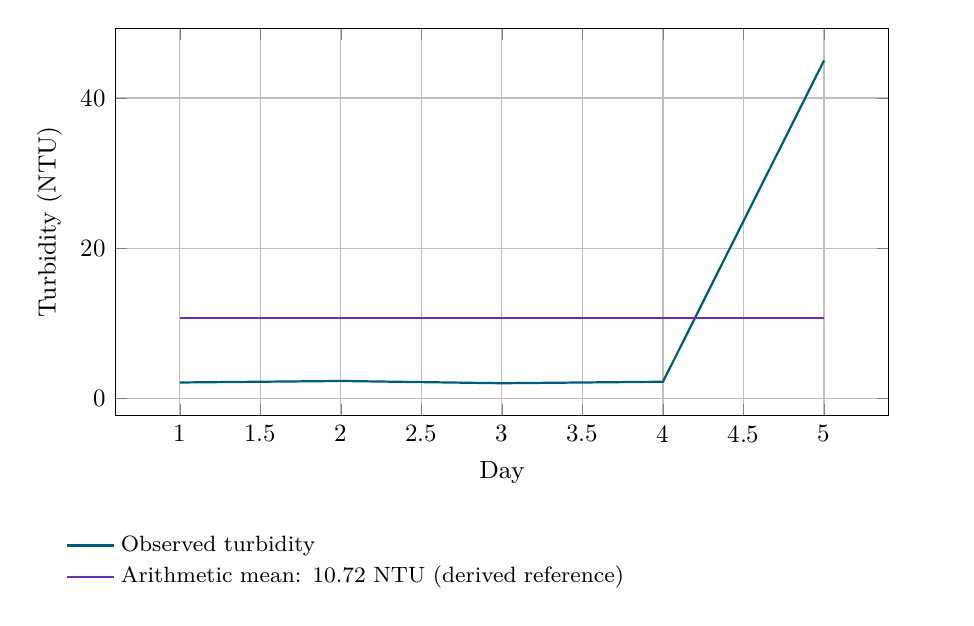
\begin{tikzpicture}
\begin{axis}[width=0.94\linewidth,
height=6.5cm,
scale only axis=false,
grid=major,
tick label style={font=\small},
label style={font=\small},
xlabel={Day},
ylabel={Turbidity (NTU)},
legend style={font=\footnotesize,draw=none,at={(0.5,-0.28)},anchor=north,legend columns=1,text width=0.85\linewidth,align=left},
unbounded coords=jump,
scaled ticks=false]
\addplot[color=pcd1,thick,mark=none] coordinates {(1,2.1) (2,2.3) (3,2) (4,2.2) (5,45)};
\addlegendentry{Observed turbidity}
\addplot[color=pcd2,thick,mark=none] coordinates {(1,10.72) (5,10.72)};
\addlegendentry{Arithmetic mean: 10.72 NTU (derived reference)}

\end{axis}
\end{tikzpicture}
\end{center}

\medskip

The sample median in \hyperref[material-6d5fa31e73ffef971b33d0c8739f99ead33a058f31776eb21eb22e1dff19eed2]{Eq.~\ref*{material-6d5fa31e73ffef971b33d0c8739f99ead33a058f31776eb21eb22e1dff19eed2}} uses the middle of the ordered observations. The odd- and even-size calculations in \hyperref[material-f1fe4c2609351f7c7a3495c937a29b3dc760b89a3cfc796fcc8419c2db4ecee5]{Eq.~\ref*{material-f1fe4c2609351f7c7a3495c937a29b3dc760b89a3cfc796fcc8419c2db4ecee5}} and \hyperref[material-6f33d16d4973ae7fa1d8b2e1ec016043bc8b322aff2d90163ba052eeb3dc4302]{Eq.~\ref*{material-6f33d16d4973ae7fa1d8b2e1ec016043bc8b322aff2d90163ba052eeb3dc4302}} specify the convention explicitly. This gives a summary resistant to changes in a few extreme magnitudes while preserving the full observations for interpretation. An extreme result remains scientifically relevant: its origin can be investigated alongside the central summary.


\par\medskip
\noindent\begin{minipage}{\linewidth}
\refstepcounter{equation}\label{material-6d5fa31e73ffef971b33d0c8739f99ead33a058f31776eb21eb22e1dff19eed2}
\noindent\textbf{Eq.~\ref*{material-6d5fa31e73ffef971b33d0c8739f99ead33a058f31776eb21eb22e1dff19eed2}.} Sample median with explicit odd- and even-sample conventions and complete rank notation.\par\nopagebreak
\begin{center}\begin{adjustbox}{max width=\linewidth}$\displaystyle \tilde{x}=\begin{cases}x_{((n+1)/2)}, & n\text{ odd}\\\frac{x_{(n/2)}+x_{(n/2+1)}}{2}, & n\text{ even}\end{cases}$\end{adjustbox}\end{center}

\par\noindent\textbf{Symbols}

\par\noindent\textbf{x̃} Sample median: the center of the sorted observations.

\par\noindent\textbf{x\ensuremath{{}_{(}}\ensuremath{{}_j}\ensuremath{{}_{)}}, n} Observation at sorted position j; n is the sample size.

\end{minipage}\par
\medskip

\par\medskip
\noindent\begin{minipage}{\linewidth}
\refstepcounter{equation}\label{material-f1fe4c2609351f7c7a3495c937a29b3dc760b89a3cfc796fcc8419c2db4ecee5}
\noindent\textbf{Eq.~\ref*{material-f1fe4c2609351f7c7a3495c937a29b3dc760b89a3cfc796fcc8419c2db4ecee5}.} Worked middle-ranked value for an odd number of observations.\par\nopagebreak
\begin{center}\begin{adjustbox}{max width=\linewidth}$\displaystyle \tilde{x}=x_{(3)}=2.2\;\mathrm{NTU}$\end{adjustbox}\end{center}

\par\noindent\textbf{Symbols}

\par\noindent\textbf{x̃} Median turbidity of five observations, in NTU.

\par\noindent\textbf{x\ensuremath{{}_{(}}\ensuremath{{}_3}\ensuremath{{}_{)}}} Third sorted value: the middle observation 2.2 NTU.

\end{minipage}\par
\medskip

\par\medskip
\noindent\begin{minipage}{\linewidth}
\refstepcounter{equation}\label{material-6f33d16d4973ae7fa1d8b2e1ec016043bc8b322aff2d90163ba052eeb3dc4302}
\noindent\textbf{Eq.~\ref*{material-6f33d16d4973ae7fa1d8b2e1ec016043bc8b322aff2d90163ba052eeb3dc4302}.} Worked midpoint of the two central observations for an even sample size.\par\nopagebreak
\begin{center}\begin{adjustbox}{max width=\linewidth}$\displaystyle \tilde{x}=\frac{2.1+2.2}{2}=2.15\;\mathrm{NTU}$\end{adjustbox}\end{center}

\par\noindent\textbf{Symbols}

\par\noindent\textbf{x̃} Median turbidity of four observations, in NTU.

\par\noindent\textbf{2.1, 2.2} Two middle sorted observations; their mean is 2.15 NTU.

\end{minipage}\par
\medskip

The lead example compares arithmetic and median summaries of the same observations (\hyperref[material-215dc13cafa4df85f0d0994d821642b077eec3a5162a3eb118cc84b7406e9a81]{Eq.~\ref*{material-215dc13cafa4df85f0d0994d821642b077eec3a5162a3eb118cc84b7406e9a81}}, \hyperref[material-c5376af3aa8ad80ad30c28da59297052dba552e1bdece4340c2bbebd40baeb32]{Eq.~\ref*{material-c5376af3aa8ad80ad30c28da59297052dba552e1bdece4340c2bbebd40baeb32}}); \hyperref[material-a9174094c1a1558f936dae4b2fa1b18f5187e9df86ca746cd05f30135ec88923]{Listing~\ref*{material-a9174094c1a1558f936dae4b2fa1b18f5187e9df86ca746cd05f30135ec88923}} supplies the optional reproduction. The chapter's unifying choice is therefore scientific: preserve an additive total, a multiplicative factor, an equal-amount rate calculation, or an ordered centre. Reporting that choice and its rationale makes the summary useful. The next level adds a description of how widely the observations vary around their centre.


\par\medskip
\noindent\begin{minipage}{\linewidth}
\refstepcounter{equation}\label{material-215dc13cafa4df85f0d0994d821642b077eec3a5162a3eb118cc84b7406e9a81}
\noindent\textbf{Eq.~\ref*{material-215dc13cafa4df85f0d0994d821642b077eec3a5162a3eb118cc84b7406e9a81}.} Arithmetic concentration summary for the authored lead observations.\par\nopagebreak
\begin{center}\begin{adjustbox}{max width=\linewidth}$\displaystyle \bar{x}=3.52\;\symup{\mu}\mathrm{g/L}$\end{adjustbox}\end{center}

\par\noindent\textbf{Symbols}

\par\noindent\textbf{\ensuremath{\bar{x}}} Arithmetic mean of five equally weighted lead concentrations.

\par\noindent\textbf{µg/L} Micrograms per litre: the observed arithmetic concentration summary is 3.52 µg/L. Safety thresholds require separate application-specific criteria.

\end{minipage}\par
\medskip

\par\medskip
\noindent\begin{minipage}{\linewidth}
\refstepcounter{equation}\label{material-c5376af3aa8ad80ad30c28da59297052dba552e1bdece4340c2bbebd40baeb32}
\noindent\textbf{Eq.~\ref*{material-c5376af3aa8ad80ad30c28da59297052dba552e1bdece4340c2bbebd40baeb32}.} Median of the same lead observations, obtained from their ordered centre.\par\nopagebreak
\begin{center}\begin{adjustbox}{max width=\linewidth}$\displaystyle \tilde{x}=0.7\;\symup{\mu}\mathrm{g/L}$\end{adjustbox}\end{center}

\par\noindent\textbf{Symbols}

\par\noindent\textbf{x̃} Middle sorted lead concentration in this sample. Safety thresholds are specified separately for the intended application.

\par\noindent\textbf{µg/L} Micrograms per litre: median 0.7 µg/L.

\end{minipage}\par
\medskip

\par\medskip
\Needspace{8\baselineskip}
\refstepcounter{listing}\label{material-a9174094c1a1558f936dae4b2fa1b18f5187e9df86ca746cd05f30135ec88923}
\noindent\textbf{Listing~\ref*{material-a9174094c1a1558f936dae4b2fa1b18f5187e9df86ca746cd05f30135ec88923}.} Optional R reproduction of the lead mean and median comparison.\par\nopagebreak
\begin{Verbatim}[fontsize=\footnotesize,breaklines=true,breakanywhere=true]
pb <- c(0.5, 0.7, 0.6, 0.8, 15.0)
list(sorted = sort(pb), median = median(pb))
\end{Verbatim}

\par\noindent\textbf{c(...)}

Combines all five Pb concentrations into a vector, including 15.0.

\par\noindent\textbf{sort(x)}

Returns the concentrations in increasing order without discarding any.

\par\noindent\textbf{median(x)}

Returns the sample median: the middle observation here, 0.7 µg/L.

\par\noindent\textbf{list(...)}

Returns the sorted observations and median together so both are visible.

\medskip

\end{document}
